\documentclass[12pt,a4paper]{article}
\usepackage[a4paper, total={6in, 8in}]{geometry}
\usepackage{siunitx}
\usepackage{tikz}
\usepackage{authblk}
\usepackage{hyperref}
\usepackage[french]{babel}
\usepackage[T1]{fontenc}
\usepackage{lmodern}
\usepackage{graphicx}
\usepackage{pythonhighlight}
\usepackage{amsmath}
\usepackage{listings}
\usepackage{amssymb}
\usepackage[rightcaption]{sidecap}
\graphicspath{ {./figures/} }

\Urlmuskip=0mu  plus 10mu

\author{VO Van Nghia}
\author{YU Duan}
\author{PHAM Tuan Kiet}
\affil{Etudians 2ème année MIC, Institut national des sciences appliquées de Toulouse}
\title{Rapport de Projet: Traitement d'images}

\begin{document}
\maketitle
\tableofcontents

\pagebreak
\section{Introduction}
\subsection{Réseaux de neurones}
\subsubsection{Définition}
Un réseau neuronal est l’association, en un graphe plus ou moins complexe,
d’objets élémentaires, les neurones formels. Les principaux réseaux se distinguent par l’organisation du graphe
(en couches, complets, \dots), c’est-à-dire leur architecture, son niveau de complexité
(le nombre de neurones, présence ou non de boucles de rétroaction dans le réseau)
par le type des neurones (leurs fonctions de transition ou d’activation) et enfin par l’objectif visé:
apprentissage supervisé ou non, optimisation, systèmes dynamiques, \dots \cite{univ-toulouse}

\begin{figure}[h!]
  \centering
  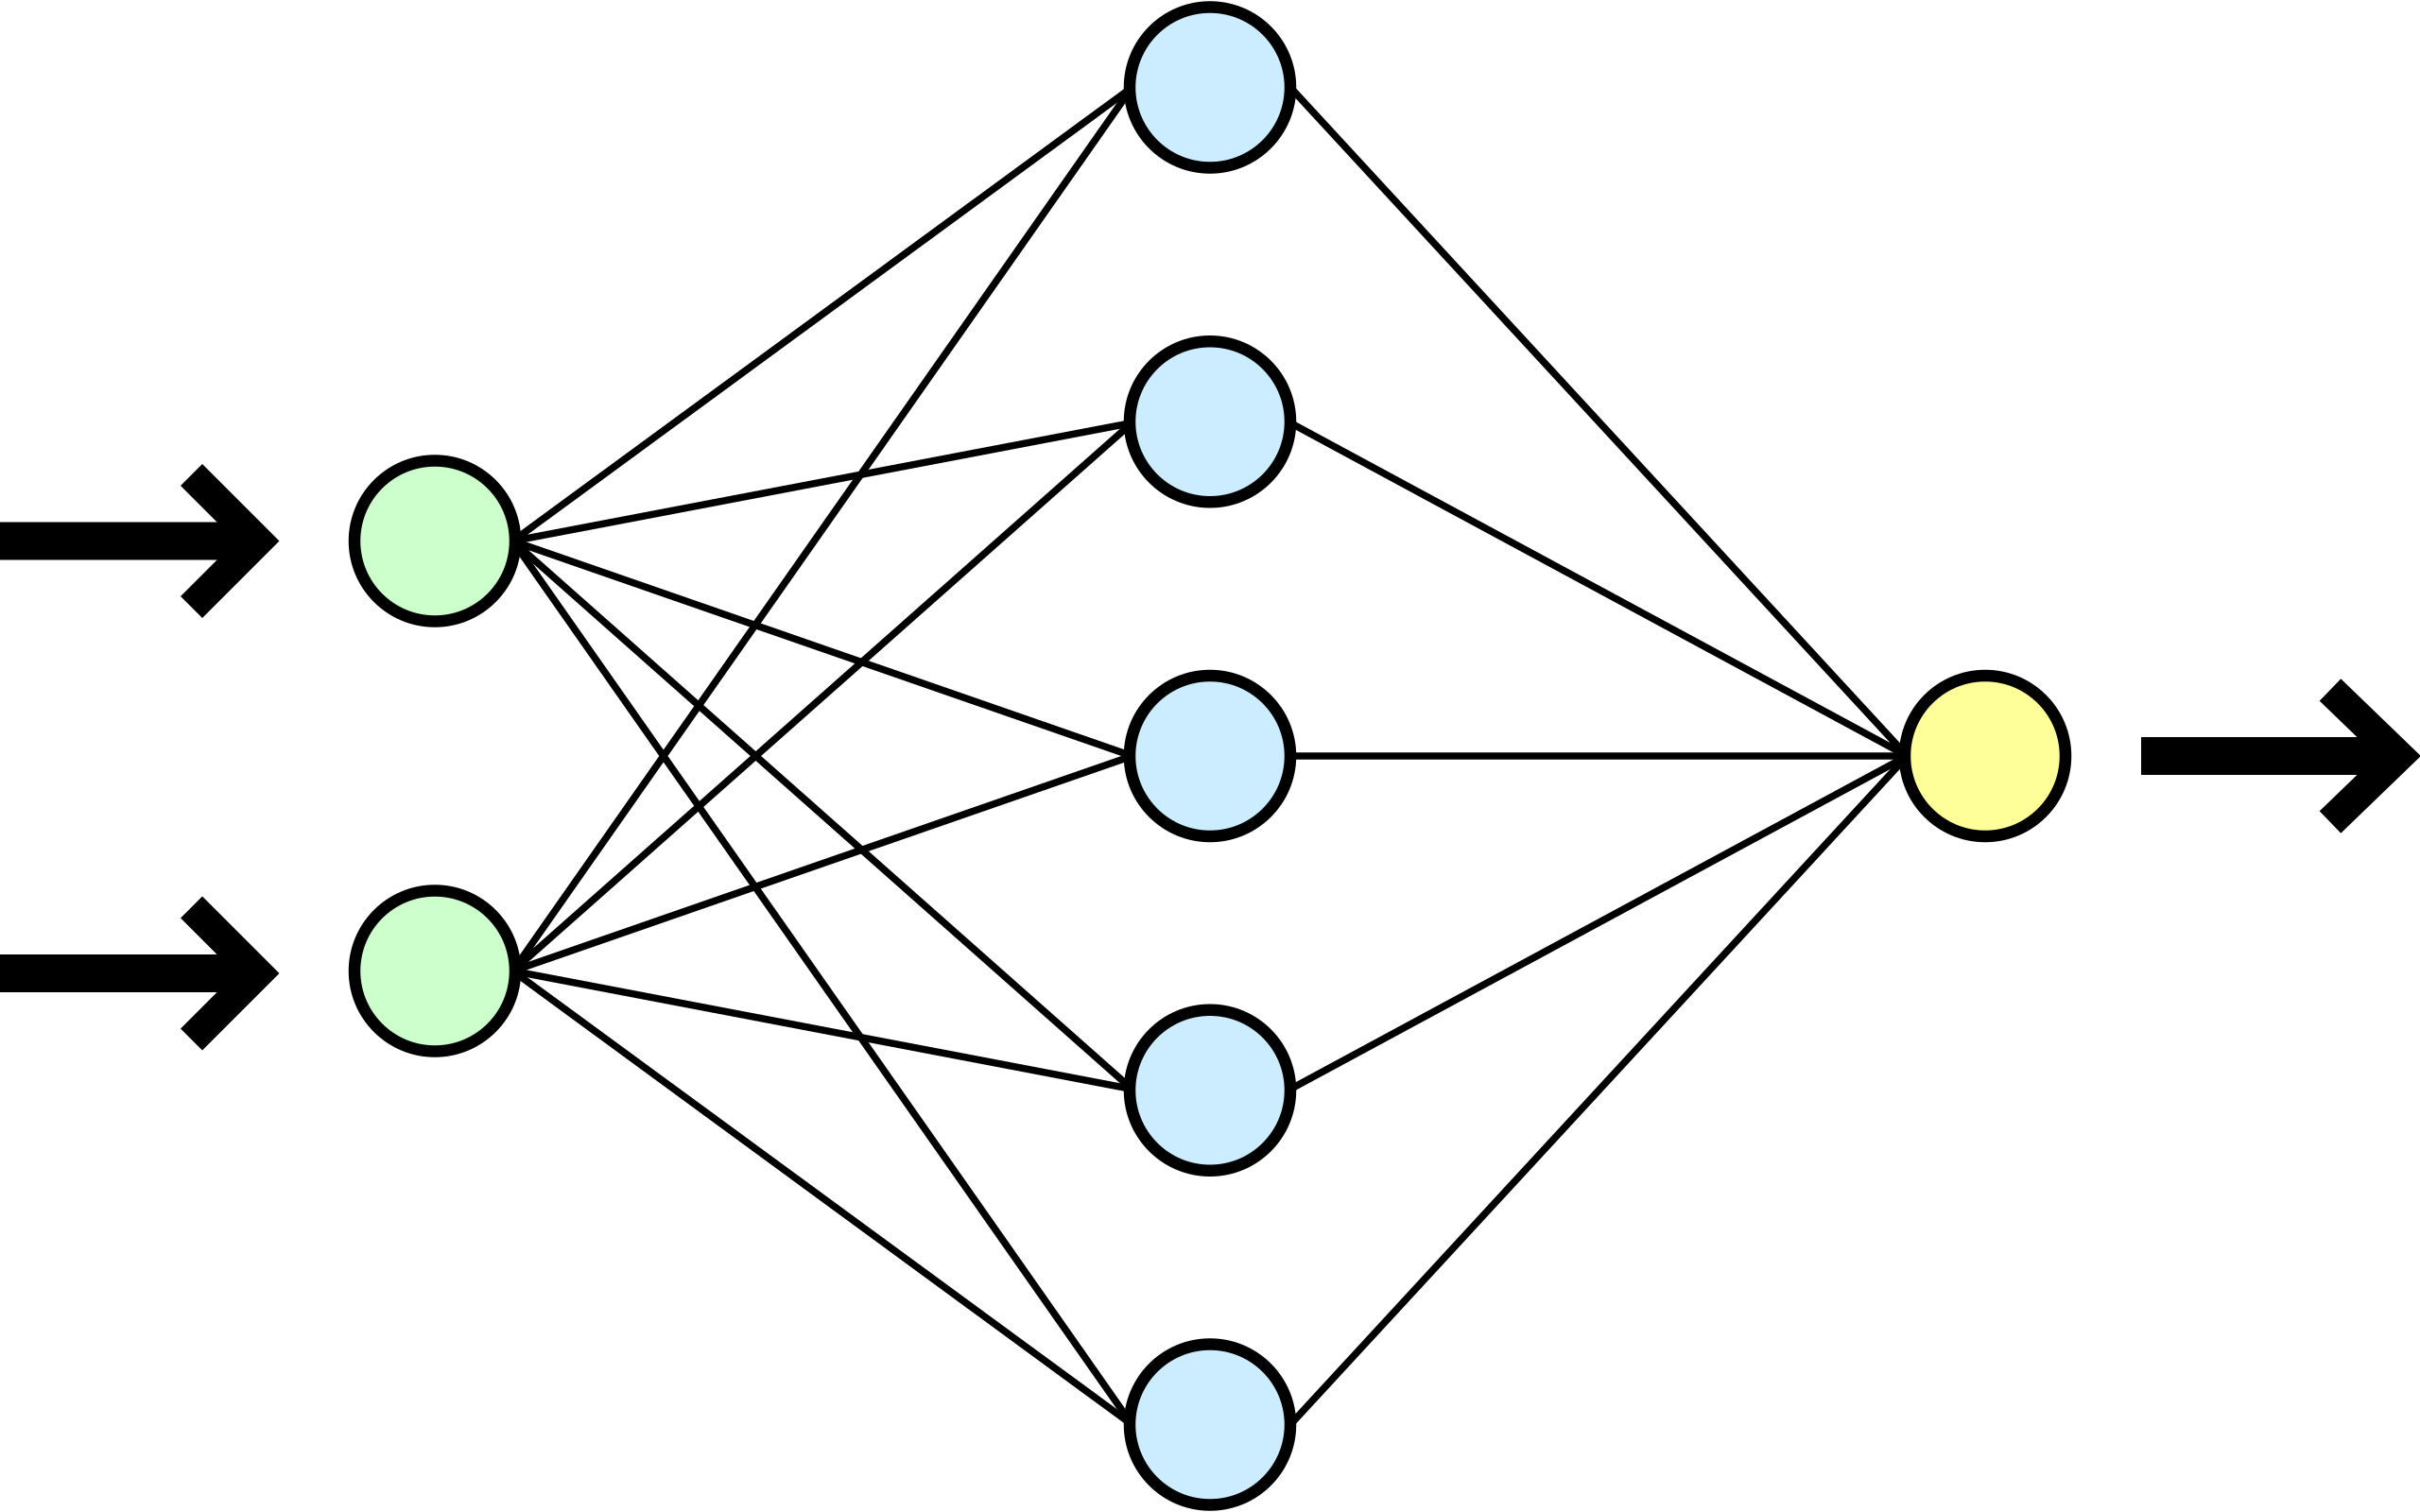
\includegraphics[width=0.5\textwidth]{Neural_network.png}
  \caption{Vue simplifiée d'un réseau artificiel de neurones}
  \label{fig:1}
\end{figure}

\subsubsection{Neurone formel}
Le neurone formel est un modèle qui se caractérise par
un état interne $s$ , des signaux d’entrée $x_{1}$, \dots,  $x_{p}$ et une fonction d’activation
$$ s=h(x_{1},\dots,x_{p})=g(\alpha_{0} + \sum_{j=1}^{p} \alpha_{j}x_{j}) = g(\alpha_{0} + \alpha' x)$$
La fonction d’activation opère une transformation d’une combinaison affine
des signaux d’entrée, $\alpha_{0}$, terme constant, étant appelé le biais du neurone.
Cette combinaison affine est déterminée par un vecteur de poids
$[\alpha_{0},\dots,\alpha_{p}]$ associé à chaque neurone et dont les valeurs sont estimées dans la phase d’apprentissage.
Ils constituent la mémoire ou connaissance répartie du réseau. \cite{univ-toulouse}

\subsection{Réseau neuronal convolutif}
Un réseau de neurones convolutifs ou réseau de neurones à convolution
est un type de réseau de neurones artificiels, dont architecture est formée par
un empilement de couches (les combinaisons des neurones formels) de traitement:\cite{wiki-cnn}
\begin{itemize}
\item[\textbullet] La couche de convolution (CONV)
\item[\textbullet] La couche de pooling (POOL)
\item[\textbullet] La couche d'activation
\item[\textbullet] La couche "entièrement connectée" (FC)
\item[\textbullet] La couche de perte (LOSS)
\end{itemize}
Dans notre projet, nous utilisons les couches suivantes: CONV, POOL et d'activation.

\section{Réalisation d'un réseau neuronal convolutif dans Python}
\subsection{Objectif}
\subsection{Récupérer et préparer les images}
Nous utilisons la base de donnée MNIST (Modified National Institute of Standards and Technology database)
pour ce projet.

\begin{figure}[h!]
  \centering
  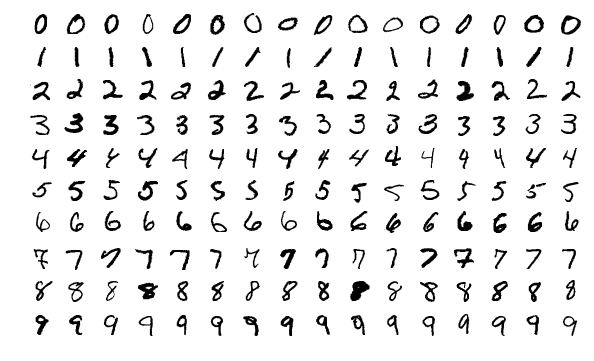
\includegraphics[width=0.5\textwidth]{mnist.png}
  \caption{Un exemple de chiffres de la base MNIST}
  \label{fig:2}
\end{figure} 
Après charger la base de donnée, on ajoute le bruit gaussien. Finallement, on met données en forme pour passer dans le réseau.
\begin{figure}[h!]
  \centering
  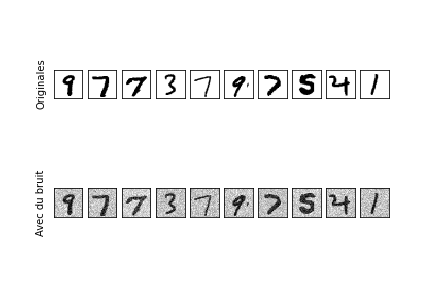
\includegraphics[width=1\textwidth]{without_result.png}
  \caption{Les images avec du bruit gaussien ajouté}
  \label{fig:3}
\end{figure}
\\
\\
\subsection{Architecture du réseau neuronal convolutif}
\begin{python}
init = Input(shape=(None, None,1))
x = Convolution2D(16, (3, 3), activation='relu', padding='same')(init) 
x = MaxPooling2D((2, 2))(x)
x = Convolution2D(32, (3, 3), activation='relu', padding='same')(x) 
x = MaxPooling2D((2, 2))(x)
x = Convolution2D(64, (3, 3), activation='relu', padding='same')(x)
x = Convolution2D(32, (3, 3), activation='relu', padding='same')(x)
x = UpSampling2D()(x)
x = Convolution2D(16, (3, 3), activation='relu', padding='same')(x)
x = UpSampling2D()(x)
x = Convolution2D(1, (3, 3), activation='relu', padding='same')(x)
\end{python}
Ci-dessus est notre code pour créer un modèle simple de notre réseau de neurones.
Chaque fonction va créer une couche comme dans la définition d'un réseau neuronal convolutif.
On va voir chaque fonction dans les parties suivantes.
\subsubsection{La couche de convolution (CONV)}
La convolution est le processus consistant à ajouter chaque élément de l'image à ses voisins immédiats,
pondéré par les éléments du noyau. C'est une forme de produit de convolution. Supposons que,
on a un image en niveaux de gris:
$\begin{bmatrix}
  1 & 2 & 3\\
  4 & 5 & 6\\
  7 & 8 & 9\\
\end{bmatrix}$
et un noyau:
$\begin{bmatrix}
  a & b & c\\
  d & e & f\\
  g & h & i\\
\end{bmatrix}$.
L'élément au coordonnée $[1, 1]$ de l'image de sortie devrait être pondéré par la combinaison de les elements entrées de la matrice de l'image, avec les poids données par le noyau comme suit :
$$\left(\begin{bmatrix}
  0 & 0 & 0 & 0 & 0\\
  0 & 1 & 2 & 3 & 0\\
  0 & 4 & 5 & 6 & 0\\
  0 & 7 & 8 & 9 & 0\\
  0 & 0 & 0 & 0 & 0\\
\end{bmatrix}
\begin{bmatrix}
  a & b & c\\
  d & e & f\\
  g & h & i\\
\end{bmatrix}\right)[1, 1] =
0\cdot a + 0\cdot b + 0\cdot c +
0\cdot d + 1\cdot e + 2\cdot f +
0\cdot g + 4\cdot h + 5\cdot i
$$
Les autres entrées devraient être pondérées de manière similaire, appliquée à tous les pixels de l'image.
De manière analogie, la fonction suivante crée deux couches successives: CONV et d'activation (ReLU).
La couche CONV est composée de $filters$ neurones formels. Chaque neurone est un noyau dont la taille
est $size$.
\begin{python}
Convolution2D(filters, size, activation='relu', padding='same')
\end{python}

\subsubsection{La couche d'activation}
La fonction d'activation est une fonction 
mathématique appliquée à
un signal en sortie d'un neurone artificiel.
Le but d'une fonction d'activation est d'ajouter une sorte de propriété non linéaire au réseau neuronal.
Sans les fonctions d'activation,
la seule opération mathématique pendant la propagation directe serait des produits scalaires entre un vecteur d'entrée et une matrice de poids.
Puisqu'un seul produit scalaire est une opération linéaire, les produits scalaires successifs ne seraient rien de plus que de multiples opérations linéaires répétées les unes après les autres.
Afin de pouvoir calculer des choses vraiment intéressantes,
les réseaux de neurones doivent être capables d'approximer les relations non linéaires des entrées aux sorties. \cite{deeplearning-academy}
\\\\
Dans notre projet, on utilise la fonction d'activation $ReLU(x) = \max(x, 0)$
\begin{SCfigure}[0.5][h]
  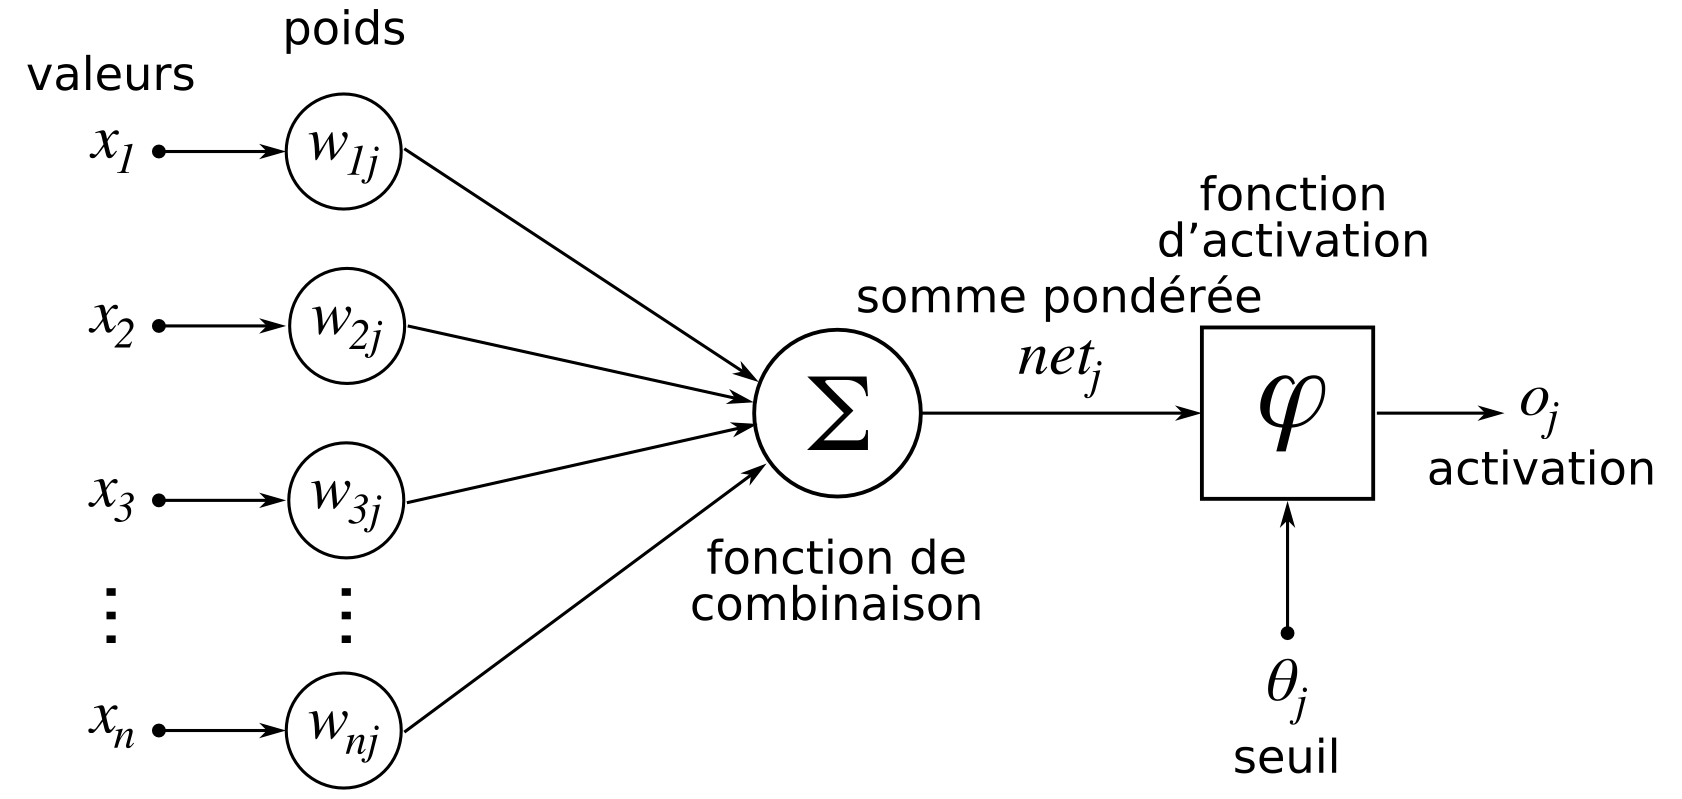
\includegraphics[width=0.6\textwidth]{neuron_model.png}
  \caption[Structure d'un neurone artificiel]{Structure d'un neurone artificiel. Le neurone calcule la somme de ses entrées puis cette valeur passe à travers la fonction d'activation pour produire sa sortie.}
  \label{fig:4}
\end{SCfigure}

\subsubsection{La couche de pooling (POOL)}
Pooling est une forme de sous-échantillonnage de l'image.
L'image d'entrée est découpée en une série de rectangles de n pixels de côté ne se chevauchant pas.
Chaque rectangle peut être vu comme une tuile.
Le signal en sortie de tuile est défini en fonction des valeurs prises par les différents pixels de la tuile.
Le pooling réduit la taille spatiale d'une image intermédiaire,
réduisant ainsi la quantité de paramètres et de calcul dans le réseau \cite{wiki-cnn}
\begin{figure}[h!]
  \centering
  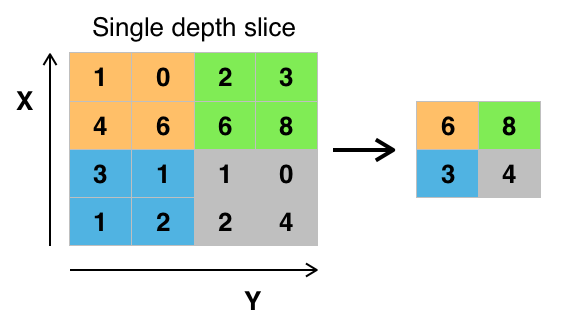
\includegraphics[width=0.5\textwidth]{max_pooling.png}
  \caption{Max pooling avec un filtre 2 × 2}
  \label{fig:5}
\end{figure}
\\
Enfin, afin d'obtenir un image de sortie ayant le même taille avec l'image d'entrée,
on utilise la fonction \lstinline{UpSampling2D} qui répète les lignes et les colonnes des données
respectivement par \lstinline{size[0]} et \lstinline{size[1]}:
$$\begin{bmatrix}
  1 & 2 & 3\\
  4 & 5 & 6\\
  7 & 8 & 9\\
\end{bmatrix} \Rightarrow
\begin{bmatrix}
  1 & 1 & 2 & 2 & 3 & 3\\
  1 & 1 & 2 & 2 & 3 & 3\\
  4 & 4 & 5 & 5 & 6 & 6\\
  4 & 4 & 5 & 5 & 6 & 6\\
  7 & 7 & 8 & 8 & 9 & 9\\
  7 & 7 & 8 & 8 & 9 & 9\\
\end{bmatrix}
$$

\subsubsection{Fonction de coût et optimisation}
Après ajouter des couches au réseau. On va choisir la fonction de coût
et le technique d'optimisation. On utilisera MSE ( Mean squared error )
comme la fonction de coût et Adam ( Adaptive moment estimation )
comme le technique d'optimisation. Finallement, on compile le model. L'architecture
de ce réseau est le diagramme suivant.
\begin{SCfigure}[0.5][h]
  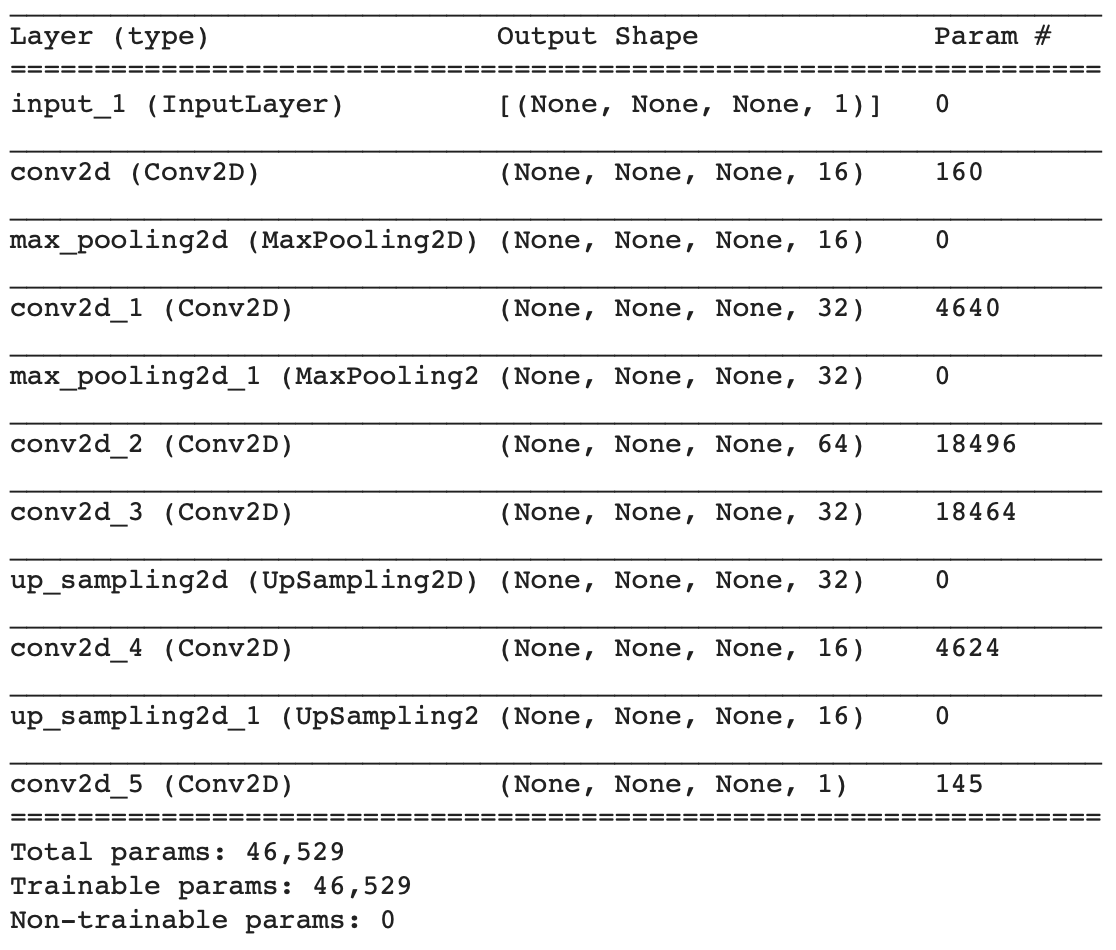
\includegraphics[width=0.7\textwidth]{architecture.png}
  \caption[Architecture d'un réseau neuronal convolutif]{Architecture d'un réseau neuronal convolutif.
  Les "Trainable params" sont les poids que on doit calculer dans le phase d'entrainement}
  \label{fig:6}
\end{SCfigure}

\subsection{Entrainement}
\subsubsection{Algorithm}
On notera $f:\theta \mapsto \mathbb{R}$ la fonction de coût, avec $\theta  = [\alpha_{0}, \dots, \alpha_{p}]$ le vecteur de poids. Dans cette partie, on va préciser comment Adam fonctionner
pour calculer les poids de réseau pour minimiser la fonction de coût. D'abord, on regarde GD ( Gradient Descent )
qui est la fondation d'Adam.\\

On rappelle que dans un repère orthonormé, le vecteur gradient $\nabla f$ pointe dans la direction où la fonction croît le plus rapidement.
Donc, dans le voisinage d'un point $\theta$, la fonction $f$ décroît le plus fortement
dans la direction opposée à celle du $\nabla f$ en $\theta$. L'algorithm GD peut être décrire dans la manière suivante: \cite{gradient-descent-wiki}
\begin{enumerate}
  \item Calcul de $\nabla f(\theta_{k})$
  \item Si $\| \nabla f(\theta_{k})\| \leqslant \epsilon$, arrêt.
  \item $\theta_{k+1} = \theta_{k} - \gamma\nabla f(\theta_{k})$
\end{enumerate}

$\gamma$ est une valeur scalaire appelée taux d'apprentissage pour déterminer le point suivant.
Mais, le problème peut survenir si le taux d'apprentissage est mal choisi.
\begin{figure}[h!]
  \centering
  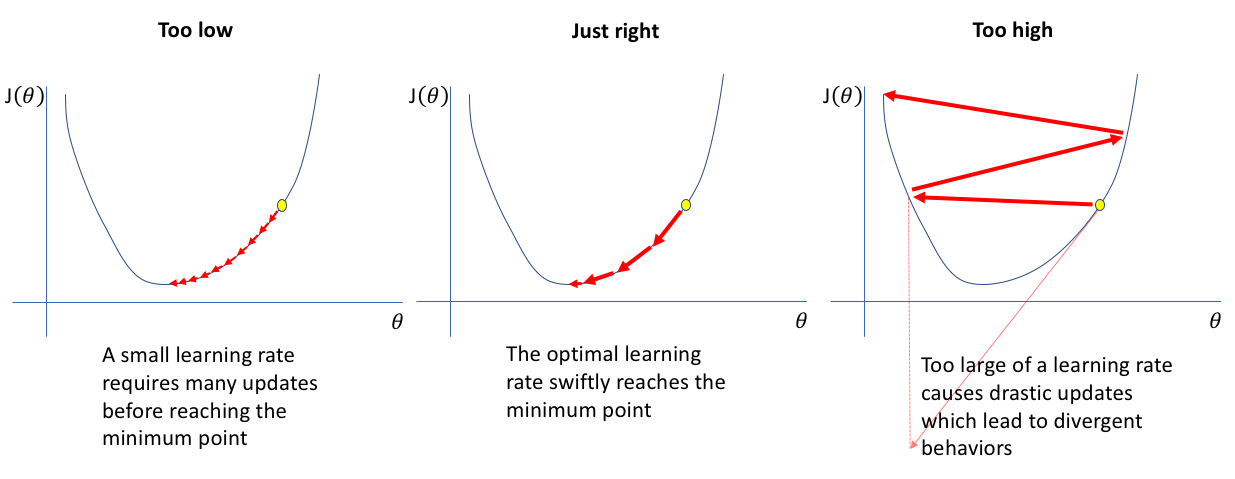
\includegraphics[width=1.0\textwidth]{learning_rate.png}
  \caption[Le taux d'apprentissage]{3 graphes montrant 3 taux d'apprentissage différents:
  trop petit (gauche), optimal (milieu), trop élevé (droite)}
  \label{fig:7}
\end{figure}

Adam résout ce problème par calcule des taux d'apprentissage adaptatifs individuels pour
différents poids.

\subsubsection{Réalisation}
\begin{python}
model.fit(y_train_ext, x_train_ext,
          batch_size=batch_size,
          epochs=epochs,
          verbose=1,
          validation_data=(y_test_ext, x_test_ext))
\end{python}

\lstinline{y_train_ext} est les images d'entrées avec du bruit gaussien,
\lstinline{x_train_ext} est les image originals. On a besion de \lstinline{validation_data} pour
éviter les problèmes concernant "overfiting". \lstinline{Epochs} est le nombre de pas de descente dans l'optimisation,
et \lstinline{batch_size} est un nombre d'échantillons traités avant la mise à jour du modèle.
\begin{figure}[h!]
  \centering
  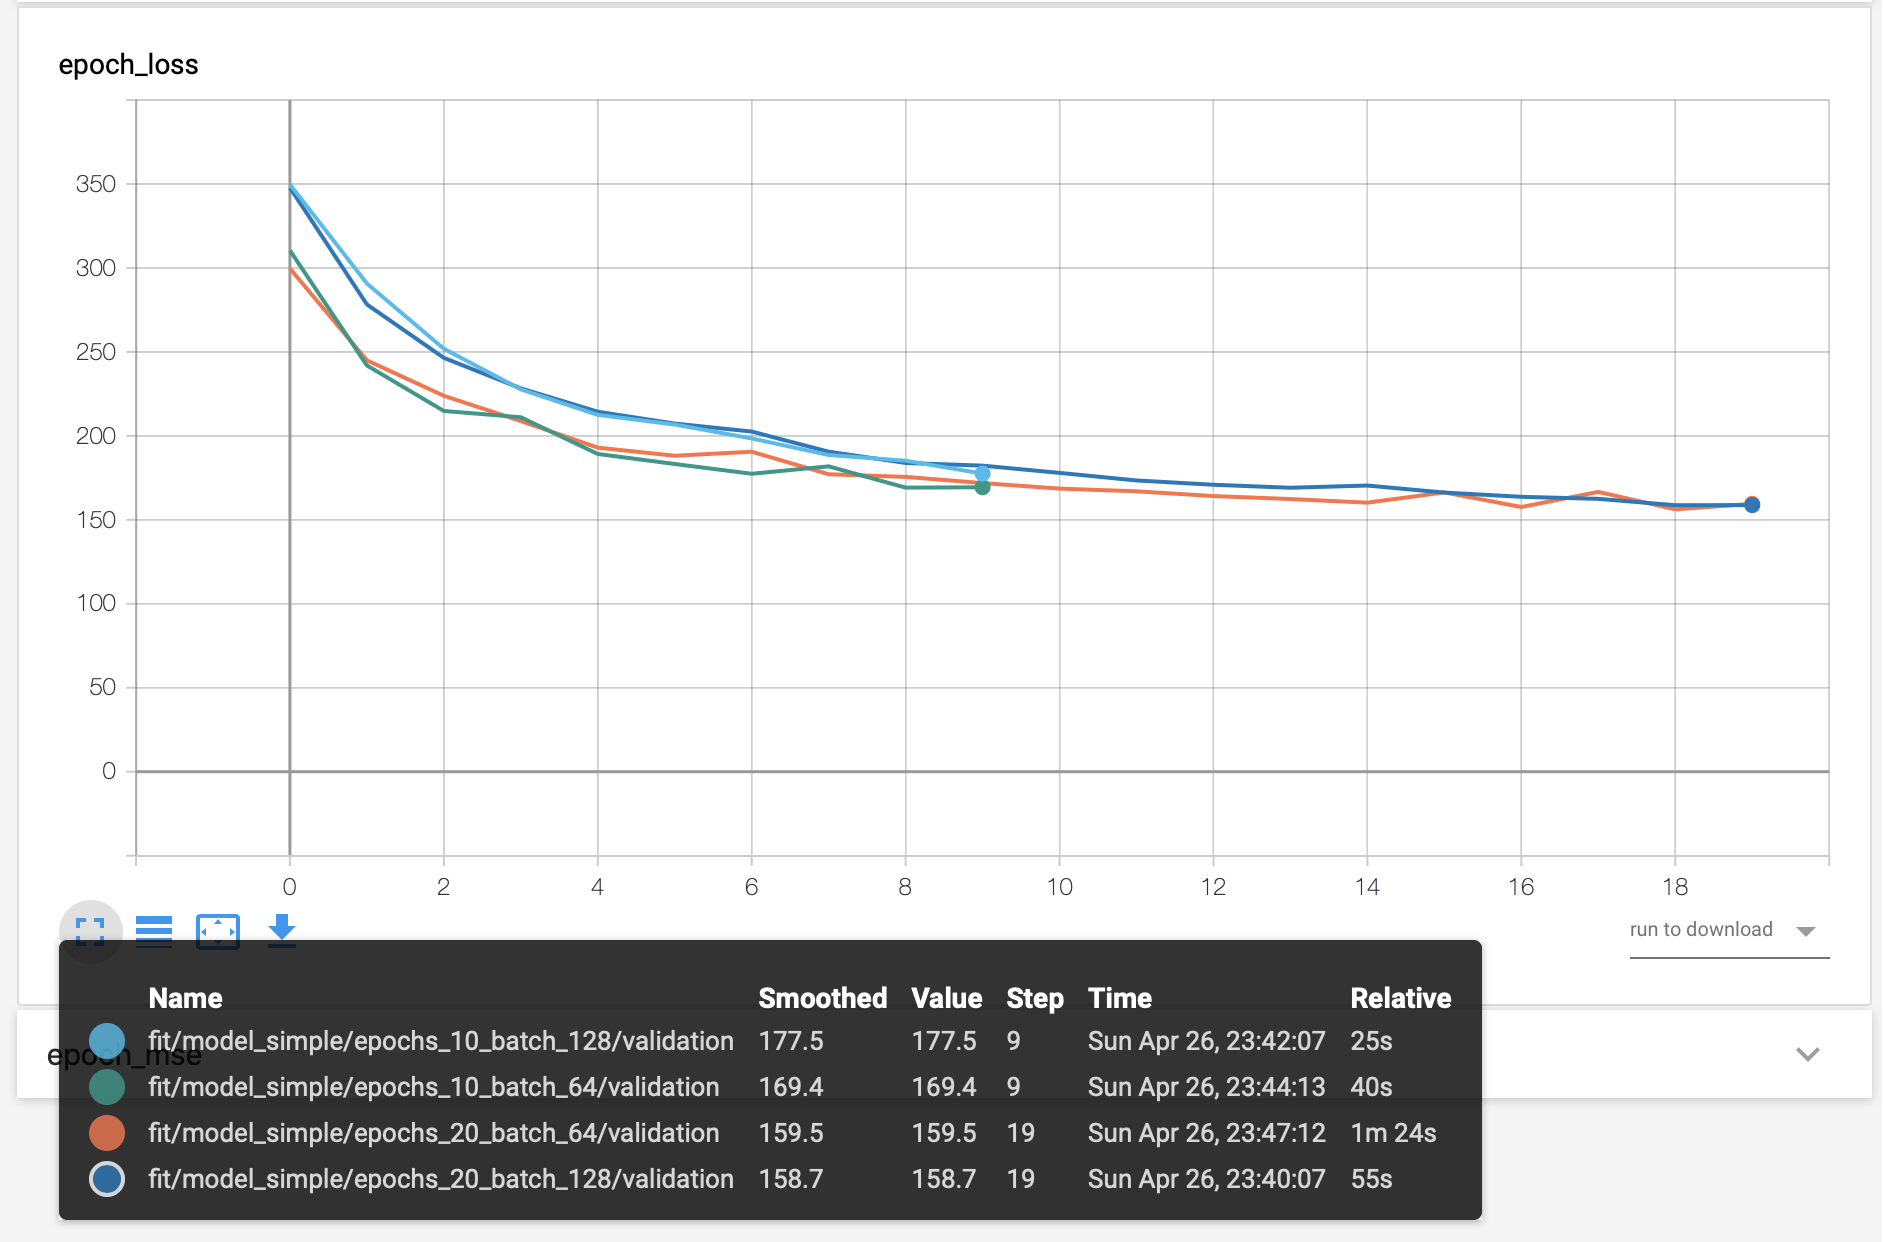
\includegraphics[width=0.9\textwidth]{epochs_batch.png}
  \caption[Epochs et \lstinline{batch_size}]{L'impact d'epochs et de \lstinline{batch_size} sur la fonction de coût}
  \label{fig:8}
\end{figure}

\begin{figure}[h!]
  \centering
  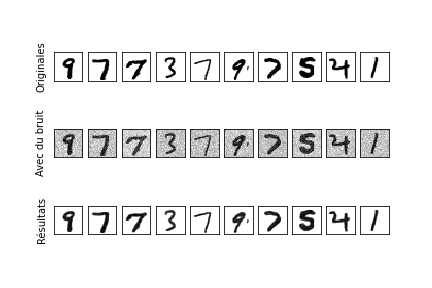
\includegraphics[width=0.8\textwidth]{model_simple.png}
  \caption{Résultat de réseau simple avec epochs = 20 et \lstinline{batch_size} = 64}
  \label{fig:9}
\end{figure}

\section{Autre architecture pour le réseau neuronal convolutif}
\subsection{Architecture linéaire}

\pagebreak
\begin{thebibliography}{9}

  \bibitem{univ-toulouse} \url{https://www.math.univ-toulouse.fr/~besse/Wikistat/pdf/st-m-app-rn.pdf}

  \bibitem{wiki-cnn} \url{https://fr.wikipedia.org/wiki/Réseau_neuronal_convolutif/}
  \bibitem{deeplearning-academy} \url{https://www.deeplearning-academy.com/p/ai-wiki-activation-functions}
  \bibitem{gradient-descent-wiki} \url{https://fr.wikipedia.org/wiki/Algorithme_du_gradient}
\end{thebibliography}
\end{document}